Detta projekt ämnat till att utveckla en Raviolimaskin. Ravioli är en traditionell italiensk maträtt bestående av rundor eller kvadratiska pastadeg med fyllning \cite{engproc}. Fyllningen kan bestå av till example köttfärs, skinka och ost. Raviolin serveras ofta i en tomatsås eller köttfärssås. Vegetarisk ravioli kan exemplvis fyllas med purjiolök eller spenat.\medskip

Att laga Ravioli hemma har varit jobbigt och tidskrävande. Det tar för mycket tid att fylla på en ravioli deg(utkavlade deg) och resultaten inte blir likadan för alla kuddar.\medskip

Det finns olika typer av Raviolimaskiner på markanden just nu. En typ av Raviolimaskin som visas på figur ~\ref{ravioli}, är en degform som underlättar processen men det mesta görs manuellt.\medskip

	\begin{figure}[h]
		\begin{center}
			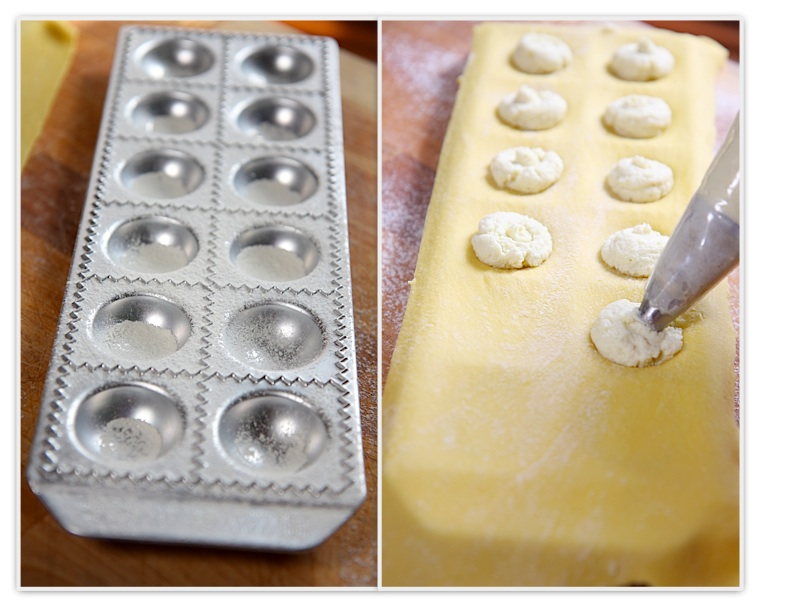
\includegraphics[scale=0.5]{images/raviolimoldwithfilling.jpg}
			\caption{Raviolimaskin}
			\label{ravioli}	
		\end{center}
	\end{figure}
Den andra typen är väldigt stor och priset är högt som medför att det inte kan användas av hushåll, se figur ~\ref{pastamaskin}.
 		\begin{figure}[h]
 			\begin{center}
 				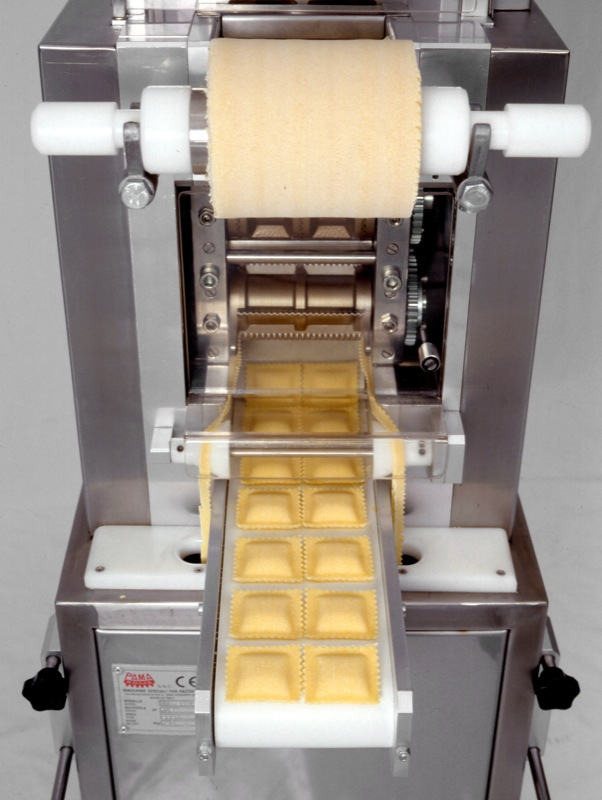
\includegraphics[scale=3]{images/pastamachine.jpg}
 				\caption{Industriell Pasta-/Raviolimaskin}
 				\label{pastamaskin}	
 			\end{center}
 		\end{figure}

Idén bakom projektet baseras på behovet av en Raviolimaskin som är lite mindre i storleken. Tanken är att man utvecklar en liten och bilig Raviolimaskin som kan vara användbar hemma.		